\chapter{Implementation}

\section{Working-Methodology}

In the events of initiation of an audio session, the system will go through the
following steps in order to successfully start streaming:\\

\begin{itemize}
    \item  The first step of course involves pointing to the media the user wishes to play.
 This involves any kind of Audio / Video source from any of the compatible providers 
 ex: Spotify, YouTube, Gaana, etc.
    \item  Time to pass the Gems ! Next , choose the client to share the Content link to.
  This will send it to the STUN / TURN servers to successfully reach the target device
    \item  The  middleware server helps in
 case of any NAT related issues and delivers the content to the correct device associated with you.
    \item  The  middleware server helps in
 case of any NAT related issues and delivers the content to the correct device associated with you.
    \item Finally the content reaches your intended device.
It parses, identifies and resolves the data, fetches the media content 
from the corresponding service and proceeds to play it. Handling the audio buffer over to the Hi-Res DAC .
    \item The Hi-Res DAC converts the binary audio buffer into a high precision analog sound signal.
 This signal is handed over to a Hi-Fi Class AB 15 watt Audio Amplifier.
    \item The Hi-Res DAC converts the binary audio buffer into a high precision analog sound signal.
 This signal is handed over to a Hi-Fi Class AB 15 watt Audio Amplifier.
    \item Finally the Hi-Fi Class AB amplifier drives the 2.4 Inch speakers producing your awaited tune.
    
\end{itemize}

 











\begin{figure}[H]
  \caption{Design}
  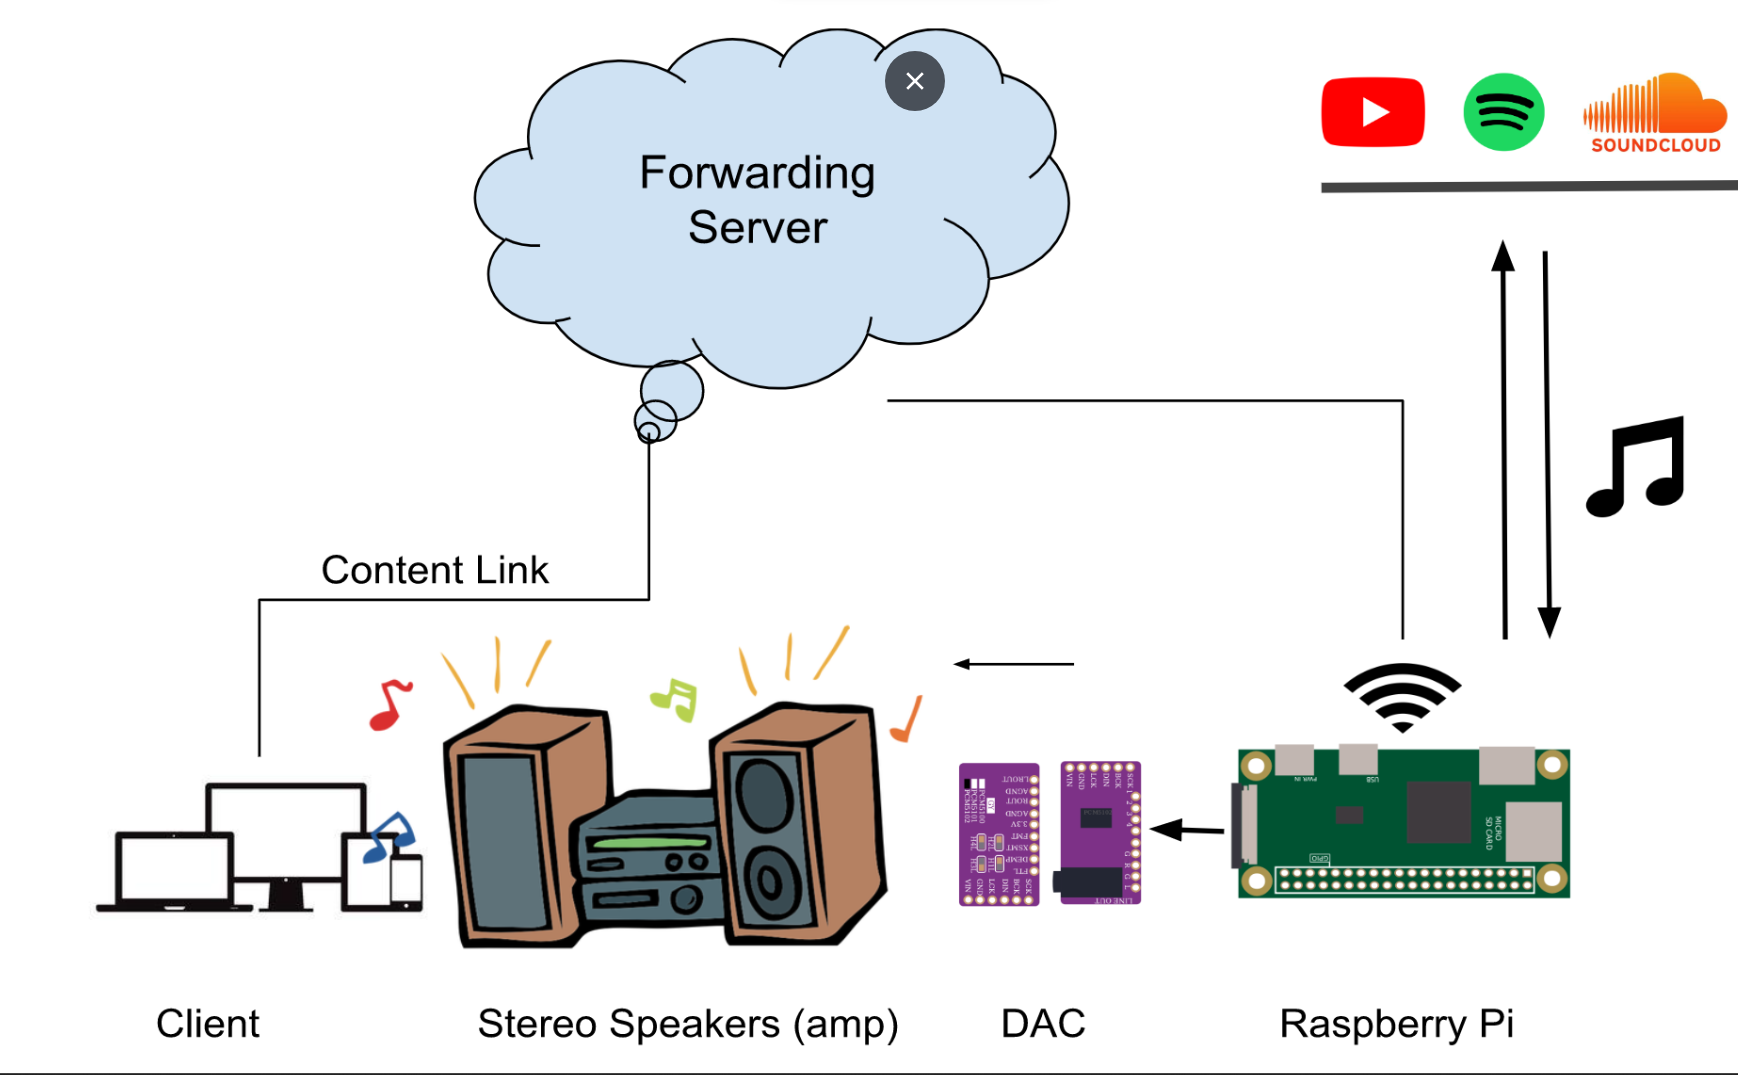
\includegraphics[scale=.4]{./implement.png}
  \\[0.2in]
\end{figure}


\section{Database Connection}
Once the library is installed, you can use the following code to create a connection to a MySQL database:\\
\begin{verbatim}
const mysql = require('mysql2');
const connection = mysql.createConnection({
  host: 'localhost',
  user: 'your-username',
  password: 'your-password',
  database: 'your-database'
});
connection.connect(function(err) {
  if (err) throw err;
  console.log('Connected to the database!');
});
\end{verbatim}


%Paste your code(limited to 5 pages)